\section*{Exercises}

\begin{problem}
  Read \emph{The Secret of Raising Smart Kids} by Carol Dweck and write a few paragraphs about what you learned and how it may help you be successful in proof-based math class.
\end{problem}

\begin{solution}
Not Interested.
\end{solution}


\begin{problem}
  Explain the error in the following "proof" that $2 = 1$. \\
  Let $x = y$. Then,

\begin{align}
x^2 &= xy \\
x^2 - y^2 &= xy - y^2 \\
(x+y)(x-y) &= y(x-y) \\
x+y &= y \\
2y &= y \\
2 &= 1
\end{align}
\end{problem}

\begin{solution}
  Since $x = y$, $x-y = 0$ and therefore, we cannot divided by $x-y$ in step $3$ to get $x+y = y$ from $(x+y)(x-y) = y(x-y)$. Thus, solved.
\end{solution}


\begin{problem}
  Suppose that $m$ and $n$ are positive odd integers. Using $2 \times 1$ dominos,

  (a) Does there exist a perfect cover of the $m \times n$ chessboard?

  (b) If I remove 1 square from the $m \times n$ chessboard, will it have a perfect cover?
\end{problem}

\begin{solution}[a]
  In this case, there are $m \times n$ cells on the board which is an odd number. Since each domino covers only $2$ cells, the total number of cells covered will always be even.

  Hence, no perfect cover exists.
\end{solution}

\begin{scratch}[b]
  Let us take $3 \times 3$ chessboard. There are $9$ cells on the board. Without loss of generality, let us say there are $4$ white cells and $5$ black cells.

  Since a domino always covers $1$ white and $1$ black cell, the number of white and black cell must be equal for a perfect cover.

  Let us remove a black cell from the above chessboard. Now there are $4$ white cells and $4$ black cells.

  Checking all $5$ black squares for removal, we find that we have a cover in every case.
\end{scratch}

\begin{solution}[b]
  Let us assume that the board has $x$ white cells and $x+1$ black cells.
	Note: If it is not the case, we can always swap the colors and have the same setup.

	Since each domino must cover exactly $1$ white and $1$ black cell, we must remove a black cell to have a perfect cover.

	In this scenario, all the corners will have black cells since there are more black cells than white.

	Now, the question is, whether we can remove any black cell. 

	\begin{lemma}\label{even_chessboard}
		For every chessboard of size $m \times n$, there exists a cover if either $m$ or $n$ is even.
	\end{lemma}

	\begin{proof}
		Let us assume that $m$ is even. We can always turn the board if $n$ is even.

		For every column, we have an even number of cells in that column as $m$ is even. Hence, we can cover that column with dominos.

		Hence, proved.
	\end{proof}


	Let us say we removed a black cell from row $r$. Now, there are two cases:
	\bigbreak

	\underline{Case 1.} $r$ is odd.

	In this case, we can divide the remaining chessboard into $(r-1) \times n$ and $(m-r) \times n$ and cover them by Lemma \ref{even_chessboard}.
	
	\textbf{Note}: In case $r = 1$ or $r = m$, we only have one remaining part. The second part is empty and thus, requires no cover.
	
	Since the corners are black, the left most cell of every odd row must be black because the colors are alternating. That is, all the cells in first column and rows $1, 3, 5, ..., m$ must be black.

	Since $r$ is odd, the left most cell in it must be black.
	Thus, the columns containing black cells in row $r$ are odd, i.e., cells in columns $1, 3, 5, ..., n$ and row $r$ are black.

	Thus, if we remove any black cell from row $r$
	we will have divided the row into two even sized pieces, 
	which can be covered by the dominos by Lemma \ref{even_chessboard}.

	\bigbreak
	\underline{Case 2.} $r$ is even.

	In this case, we can take rows $r-1, r, r+1$ 
	and divide the remaining chess board in $(r-2) \times n$ and $(m-r-1) \times n$ 
	and cover them by Lemma \ref{even_chessboard}.

	Since $r$ is even, all the cells in row $r$ and columns $2, 4, 8, ..., n-1$ are black.
	
	Let us say we remove the cell in column $c$. Now, we can take column $c-1, c$ and $c+1$, 
	and divide the rest of cells into chess boards of sizes $(c-2)\times 3$ and $(n-c-1) \times 3$. Since $c$ is even, therefore, $c-2$ and $n-c-1$ are even as well.
	
	Thus, we can cover these boards using Lemma \ref{even_chessboard}.

	Now, for the remainig $3 \times 3$ board without its center, we can cover it like this:
	\bigbreak

	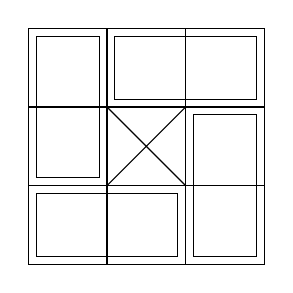
\begin{tikzpicture}
		\foreach \x in {0,1,2}
		\foreach \y in {0,1,2}
		{
			\draw (\x,\y) -- (\x+1,\y) -- (\x+1,\y+1) -- (\x,\y+1) -- (\x,\y);
		}

		\draw (1,1) -- (2,2) -- (1,2) -- (2,1);

		\draw (0.1,0.1) -- (1.9,0.1) -- (1.9,0.9) -- (0.1,0.9) -- (0.1,0.1);
		\draw (2.1,0.1) -- (2.9,0.1) -- (2.9, 1.9) -- (2.1,1.9) -- (2.1,0.1);
		\draw (2.9,2.1) -- (2.9,2.9) -- (1.1,2.9) -- (1.1,2.1) -- (2.9,2.1);
		\draw (0.1,1.1) -- (0.9,1.1) -- (0.9,2.9) -- (0.1,2.9) -- (0.1,1.1);
	\end{tikzpicture}

		Hence, proved.

\end{solution}

\begin{problem}
  The game \textbf{Tetris} is played with five different shapes -- the five shapes that can be obtained by piecing together four squares.

\bigbreak

\resizebox{\textwidth}{!}{
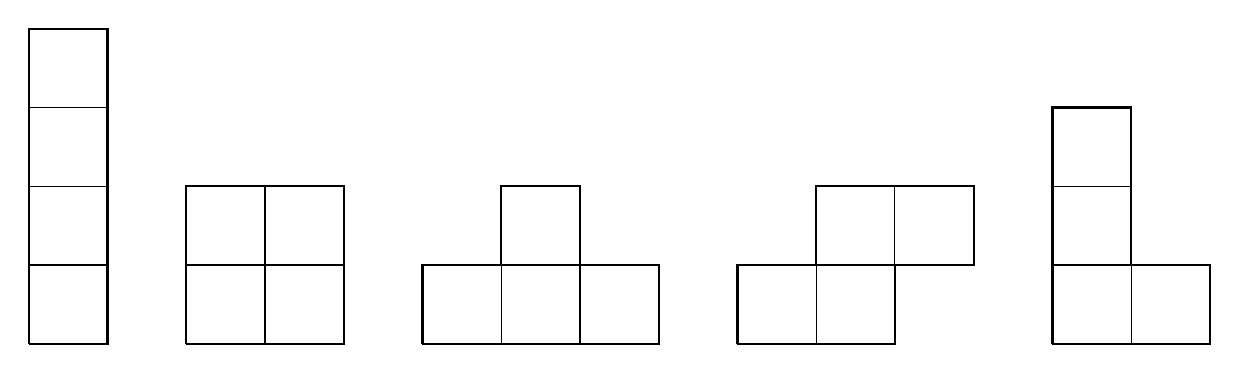
\begin{tikzpicture}
	\draw[thick] (0,0) -- (1,0) -- (1,4) -- (0,4) -- (0,0);
	\draw (0,1) -- (1,1);
	\draw (0,2) -- (1,2);
	\draw (0,3) -- (1,3);

	\draw[thick] (2,0) -- (4,0) -- (4,2) -- (2,2) -- (2,0);
	\draw (3,0) -- (3,2);
	\draw (2,1) -- (4,1);

	\draw[thick] (5,0) -- (8,0) -- (8,1) -- (7,1) -- (7,2) -- (6,2) -- (6,1) -- (5,1) -- (5,0);
	\draw (6,0) -- (6,1) -- (7,1) -- (7,0);

	\draw[thick] (9,0) -- (11,0) -- (11,1) -- (12,1) -- (12,2) -- (10,2) -- (10,1) -- (9,1) -- (9,0);
	\draw (10,0) -- (10,1) -- (11,1) -- (11,2);

	\draw[thick] (13,0) -- (13,3) -- (14,3) -- (14,1) -- (15,1) -- (15,0) -- (13,0);
	\draw (13,1) -- (14,1) -- (14,0);
	\draw (13,2) -- (14,2);
\end{tikzpicture}
}
\bigbreak

	For the questions below, we also allow these pieces to be "flipped over".

	(a) Is it possible to perfectly cover a $4 \times 5$ chessboard using each of these shapes exactly once? Prove that it is impossible, or show by example that it is possible.

	(b) Is it possible to perfectly cover an $8 \times 5$ chessboard using each of these shapes exactly twice? Prove that it is impossible, or show by example that it is possible.
\end{problem}

\begin{scratch}
	Let's color the chessboard in black and white. Here, we can see that all the shapes will cover $2$ black cells and $2$ white cells except the third shape.

	The third shape will cover either $3$ black and $1$ white cell or $1$ black and $3$ white cells.

	Therefore, if we use each shape exactly once, we will get either get a total of $11$ black and $9$ white cells or $9$ black and $11$ white cells.
\end{scratch}

\begin{solution}[a]
	Let's assume that it is possible to cover a $4 \times 5$ chessboard using these shapes exactly once.

	The chess board has exactly $10$ black and $10$ white cells in it. Each shape will take up exactly $2$ white and $2$ black cells except the third shape. 

	The third shape will either take up $3$ black and $1$ white cell or $3$ white or $1$ black cell. This is because all adjacent cells must be different color so if the center of the third shape is white, all the rest $3$ cells of that shape must be black and vice versa.

	Let's place each shape one by one. \\
	After placing the first shape, we will have $8$ black and $8$ white cells. \\
	After placing the second shape, we will have $6$ black and $6$ white cells. \\
	After placing the fourth shape, we will have $4$ black and $4$ white cells. \\
	After placing the fifth shape, we will have $2$ black and $2$ white cells.

	Now, we don't have enough white or black cells to place the third shape.
	This is a contradiction. Therefore, it is impossible to cover a $4 \times 5$ chessboard using each of these shapes exactly once.

	Hence, proved.
\end{solution}

\begin{solution}[b]
Giving an example:


\bigbreak
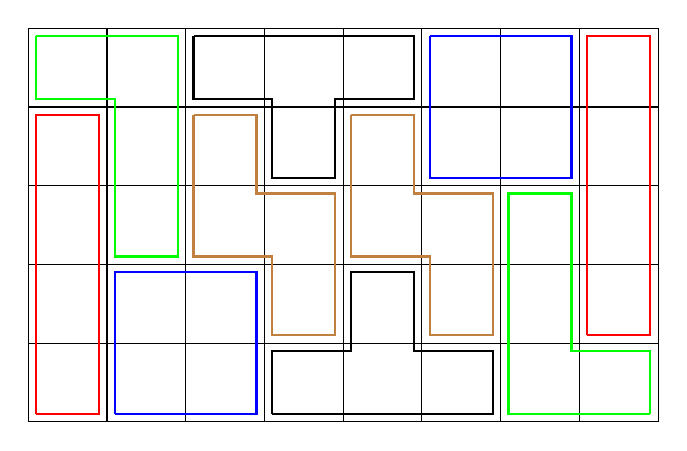
\begin{tikzpicture}
  \foreach \x in {0,1,2,3,4,5,6,7}
    \foreach \y in {0,1,2,3,4}
      {
        \draw (\x,\y) -- (\x+1,\y) -- (\x+1,\y+1) -- (\x,\y+1) -- (\x,\y);
			}

	% Long
	\draw[thick,red] (0.1,0.1) -- (0.1, 3.9) -- (0.9,3.9) -- (0.9,0.1) -- (0.1,0.1); 
	\draw[thick,red] (7.1,1.1) -- (7.1, 4.9) -- (7.9,4.9) -- (7.9,1.1) -- (7.1,1.1); 

	% Square
	\draw[thick,blue] (1.1,0.1) -- (1.1,1.9) -- (2.9,1.9) -- (2.9,0.1) -- (1.1,0.1);
	\draw[thick,blue] (5.1,4.9) -- (5.1,3.1) -- (6.9,3.1) -- (6.9,4.9) -- (5.1,4.9);

	% L-Piece
	\draw[thick,green] (0.1,4.9) -- (0.1,4.1) -- (1.1,4.1) -- (1.1,2.1) -- (1.9,2.1) -- (1.9, 4.9) -- (0.1,4.9);
	\draw[thick,green] (7.9,0.1) -- (6.1,0.1) -- (6.1, 2.9) -- (6.9, 2.9) -- (6.9, 0.9) -- (7.9, 0.9) -- (7.9, 0.1);

	% Z-Piece
	\draw[thick,brown] (2.1,3.9) -- (2.9,3.9) -- (2.9,2.9) -- (3.9,2.9) -- (3.9,1.1) -- (3.1,1.1) -- (3.1,2.1) -- (2.1,2.1) -- (2.1,3.9);
	\draw[thick,brown] (4.1,3.9) -- (4.9,3.9) -- (4.9,2.9) -- (5.9,2.9) -- (5.9,1.1) -- (5.1,1.1) -- (5.1,2.1) -- (4.1,2.1) -- (4.1,3.9);

	% T-Piece
	\draw[thick] (2.1,4.9) -- (2.1,4.1) -- (3.1,4.1) -- (3.1,3.1) -- (3.9,3.1) -- (3.9,4.1) -- (4.9,4.1) -- (4.9,4.9) -- (2.1,4.9);
	\draw[thick] (3.1,0.1) -- (3.1,0.9) -- (4.1,0.9) -- (4.1,1.9) -- (4.9,1.9) -- (4.9,0.9) -- (5.9,0.9) -- (5.9,0.1) -- (3.1,0.1);
\end{tikzpicture}

Hence, proved.
\end{solution}

\begin{problem}
	If I remove two squares of different colors from an $8 \times 8$ chessboard, must the result have a perfect square?
\end{problem}

\begin{solution}
TODO
\end{solution}

\begin{problem}
	If I remove four squares -- two white, two black -- from an $8 \times 8$ chessboard, must the result have a perfect cover?

	$\rightarrow$ If you believe a perfect cover exists, justify why.

	$\rightarrow$  If you belive a perfect cover does not need to exist, give an example of four squares that you could remove for which the result does not have a perfect cover.
\end{problem}

\begin{solution}
	TODO
\end{solution}

\begin{problem}
	In chess, a \textbf{knight} is a piece that can move two squares vertically and one square horizontally, or two squares horizontall and one square vertically.

	A \textbf{knight} can legally move to any square provided there is not another piece on that same square.

	(a) Suppose there is a knight on every square of a $7 \times 7$ chessboard. Is it possible for every one of those knights to simultaneously make a legal move?

	(b) Suppose there is a knight on every square of a $8 \times 8$ chessboard. Is it possible for every one of those knights to simultaneously make a legal move?
\end{problem}


\begin{solution}[a]
Let us color the chessboard such that there are $24$ white squares and $25$ black squares without loss of generality.

In one move, a \textbf{knight} on a white square moves to a black square and vice-verse.

Since there are more black squares than white squares, we cannot move all the knight simultaneuosly such that all of them occupy different squares after the move by Principle \ref{pigeonhole}.
\end{solution}

\begin{solution}[b]
	In the first two rows of the $8 \times 8$ chessboard, there are $8$ white squares and $8$ black squares. We can pair them up like so:
\bigbreak

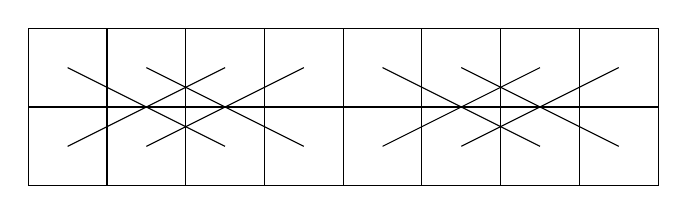
\begin{tikzpicture}
	\foreach \x in {0,1,2,3,4,5,6,7}
	\foreach \y in {0,1} {
		\draw (\x,\y) -- (\x+1,\y) -- (\x+1,\y+1) -- (\x,\y+1) -- (\x,\y);
	}
	\foreach \x in {0.5,1.5,4.5,5.5} {
		\draw (\x,1.5) -- (\x+2,0.5);
		\draw (\x+2,1.5) -- (\x,0.5);
	}
\end{tikzpicture}

This pattern can be repeat by every two rows of the board. And the knights in these places can swap positions.

Hence, proved.

\end{solution}

\begin{problem}
	Prove that if one chooses $n+1$ numbers from $\{1, 2, 3, ..., 2n\}$, it is guaranteed that two of the numbers that they choose are consecutive.

	Also, before the proof, write 2 example for $n=3$, $n=4$ and $n=5$.
\end{problem}

\begin{scratch}
	For $n=3$, we can choose $4$ numbers from $\{1, 2, 3, 4, 5, 6\}$. Let them be $1, 3, 5, 6$. Here, $5$ and $6$ are consecutive.

	For $n=4$, we can choose $5$ numbers from $\{1, 2, 3, 4, 5, 6, 7, 8\}$. Let them be $1, 3, 5, 7, 8$. Here, $7$ and $8$ are consecutive.

	For $n=5$, we can choose $6$ numbers from $\{1, 2, 3, 4, 5, 6, 7, 8, 9, 10\}$. Let them be $1, 3, 5, 7, 9, 10$. Here, $9$ and $10$ are consecutive.
\end{scratch}

\begin{solution}
	Let us define the $n$ boxes numbered $1$ to $n$.
	For each selected $x$, if $x = 2k - 1$ or $x = 2k$, put it in the box $k$.

	Thus, box $k$ will only contain two numbers: $2 \cdot k - 1$ and $2 \cdot k$. Both these numbers are consecutive.

	Since there are $n+1$ selected numbers atleast two numbers must be in the same box by Principle \ref{pigeonhole} which implies that they are consecutive.

	Hence, proved.
\end{solution}

\begin{problem}
	Assume that $n$ is a positive integer. Prove that if one selects any $n+1$ numbers from the set $\{1, 2, 3, ..., 2n\}$, then two of the selected numbers will sum to $2n+1$.
\end{problem}

\begin{solution}
	Let us define $n$ boxes numbered $1$ to $n$ such that box $i$ contains the numbers $i$ and $2n+1-i$.
	
	Thus, we will get boxes with numbers $(1, 2n), (2, 2n-1), ... (n, n+1)$. Note that the numbers in a box add up to $2n+1$.

	Now, since there are $n+1$ selected numbers atleast two numbers must be in the same box by Principle \ref{pigeonhole} which implies that they add up two $2n+1$.
\end{solution}


\begin{problem}
	Explain in your own words what the general pigeonhole princple says.
\end{problem}

\begin{solution}
	If there are $n$ objects that are placed into $m$ boxes then there is atleast one box with atleast $\lfloor \frac{n}{m} \rfloor$ items in it.
\end{solution}


\begin{problem}
	Prove that there are atleast two U.S. residents that have the same weight when rounded to the nearest \textbf{millionth} of a pound. 
\end{problem}

\begin{solution}
	A quick google search tells us that there are only $3.2$ million people over $300$ pounds in the U.S. and the population of the U.S. is $340$ million people.

	Thus, there are more than $330$ million people that weigh between $0$ and $300$ pounds.

	Let us create box for each weight with a millionth of a pound of precision. This will give us $300$ million boxes each denoting a weight with a precision of a millionth of a pound.

	Since there are more than $300$ million people in the U.S. who weigh between $0$ and $300$ pounds, by Principle \ref{pigeonhole}, we can conclude that there are atleast two people with the exact same weight when rounded to a millionth of a pound.
\end{solution}


\begin{problem}
	Determine whetehr or not the pigeonhole principle guarantees that two students at your school have the exact three leter initials.
\end{problem}

\begin{solution}
	My school had $1000$ students in each year so a total of $4000$ students.

	There are $26 \cdot 26 \cdot 26 = 17576$ unique three letter initials.

	Therefore, the pigeonhole principle doesn't guarantee that two students at my school have the same three letter initial.
\end{solution}


\begin{problem}
	Find your own real-world example of the pigeonhole principle.
\end{problem}

\begin{solution}
	There are $10,000$ engineers at my workplace. But there are only $366$ days in the year. 

	Therefore, atleast $\lfloor 10000/366 \rfloor = 27$ employees have the exact same joining anniversary.
\end{solution}

\begin{named}[Definition]
	Two integers $m$ and $n$ are said to be \emph{relatively prime} if there is no integer larger than $1$ which divides both $m$ and $n$.
\end{named}

This definition will be used in the following exercise.

\begin{problem}
Prove that if one chooses $31$ numbers from the set $\{1,2,3,...,60\}$, that two of the numbers must be relatively prime.
\end{problem}

\begin{solution}
	We can use the same method as last one. We can create $30$ boxes where each box $k$ will contain the numbers $2k-1$ and $2k$. Thus, we will get boxes that contain the numbers $(1, 2), (3, 4), (5, 6) ..., (59, 60)$. 

	Here, it is obvious that both numbers in a box are relatively prime.

	Thus, putting $31$ selected numbers in these boxes, we will get atleast one box which has atleast two numbers.

	Therefore, there are two numbers that are relatively prime.

	Hence, proved.
\end{solution}
